\documentclass[cjk,dvipdfmx,12pt,%
hyperref={bookmarks=true,bookmarksnumbered=true,bookmarksopen=false,%
colorlinks=false,%
pdftitle={第 43 回 関西 Debian 勉強会},%
pdfauthor={倉敷・のがた・佐々木},%
%pdfinstitute={関西 Debian 勉強会},%
pdfsubject={資料},%
}]{beamer}

\title{第 43 回 関西 Debian 勉強会}
\subtitle{{\scriptsize 資料}}
\author[佐々木 洋平]{{\large\bf 倉敷・のがた・佐々木}}
\institute[Debian JP]{{\normalsize\tt 関西 Debian 勉強会}}
\date{{\small 2011 年 1 月 23 日}}

%\usepackage{amsmath}
%\usepackage{amssymb}
\usepackage{graphicx}
\usepackage{moreverb}
\usepackage[varg]{txfonts}
\AtBeginDvi{\special{pdf:tounicode EUC-UCS2}}
\usetheme{Kyoto}
\def\museincludegraphics{%
  \begingroup
  \catcode`\|=0
  \catcode`\\=12
  \catcode`\#=12
  \includegraphics[width=0.9\textwidth]}
%\renewcommand{\familydefault}{\sfdefault}
%\renewcommand{\kanjifamilydefault}{\sfdefault}
\begin{document}
\settitleslide
\begin{frame}
\titlepage
\end{frame}
\setdefaultslide

\begin{frame}[fragile]
\frametitle{Agenda}

\tableofcontents

\end{frame}

\section{最近の Debian 関係のイベント}


\takahashi[40]{最近の Debian\\関係のイベント}

\takahashi[50]{squeeze}
\takahashi[50]{いよいよ\\リリース?}
\begin{frame}[fragile]
\frametitle{squeeze いよいよリリース?}

\begin{itemize}
\item リリース日程: 2 月 5 日前後, という News !!
\item RC バグも残り \textbf{39} !!
  \begin{itemize}
  \item いずれも原稿執筆時点のお話ですが.
  \end{itemize}
\centering
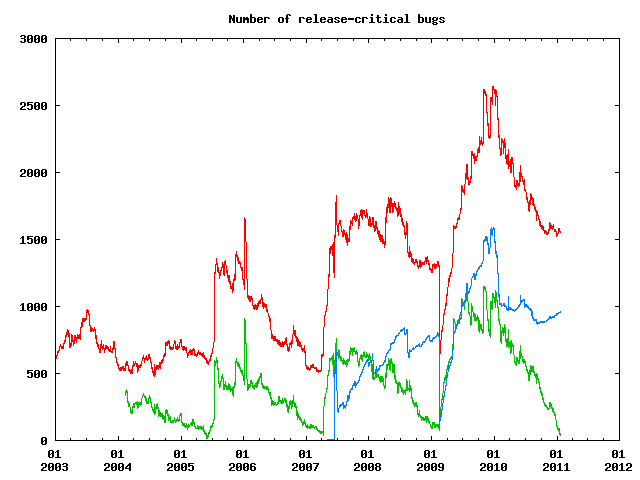
\includegraphics[width=0.55\textwidth]{./image201101/rc-status-20110123.png}
\end{itemize}
\end{frame}

\begin{frame}[fragile]
\frametitle{第 42 回関西 Debian 勉強会}

\begin{itemize}
\item 日時: 12 月 23 日
\item 於: 大阪福島区民センター
\end{itemize}

\begin{block}{内容}
  \begin{itemize}
  \item Proxmox VE の紹介 by 森山さん
  \item 2010 年を振り返る
  \end{itemize}
\end{block}
ネタ出しは随時行なっております! 皆様よろしく!!
\end{frame}

\begin{frame}[fragile]
  \frametitle{東京エリア Debian 勉強会}
  \begin{itemize}
  \item 第 71 回: 2010/12/18 開催. \\ \qquad libsane と CACert 話
  \item 第 72 回: 2010/01/15 開催. \\ \qquad Debian 勉強会アンケートシステム と Kinnect の話
  \end{itemize}
  \centering
  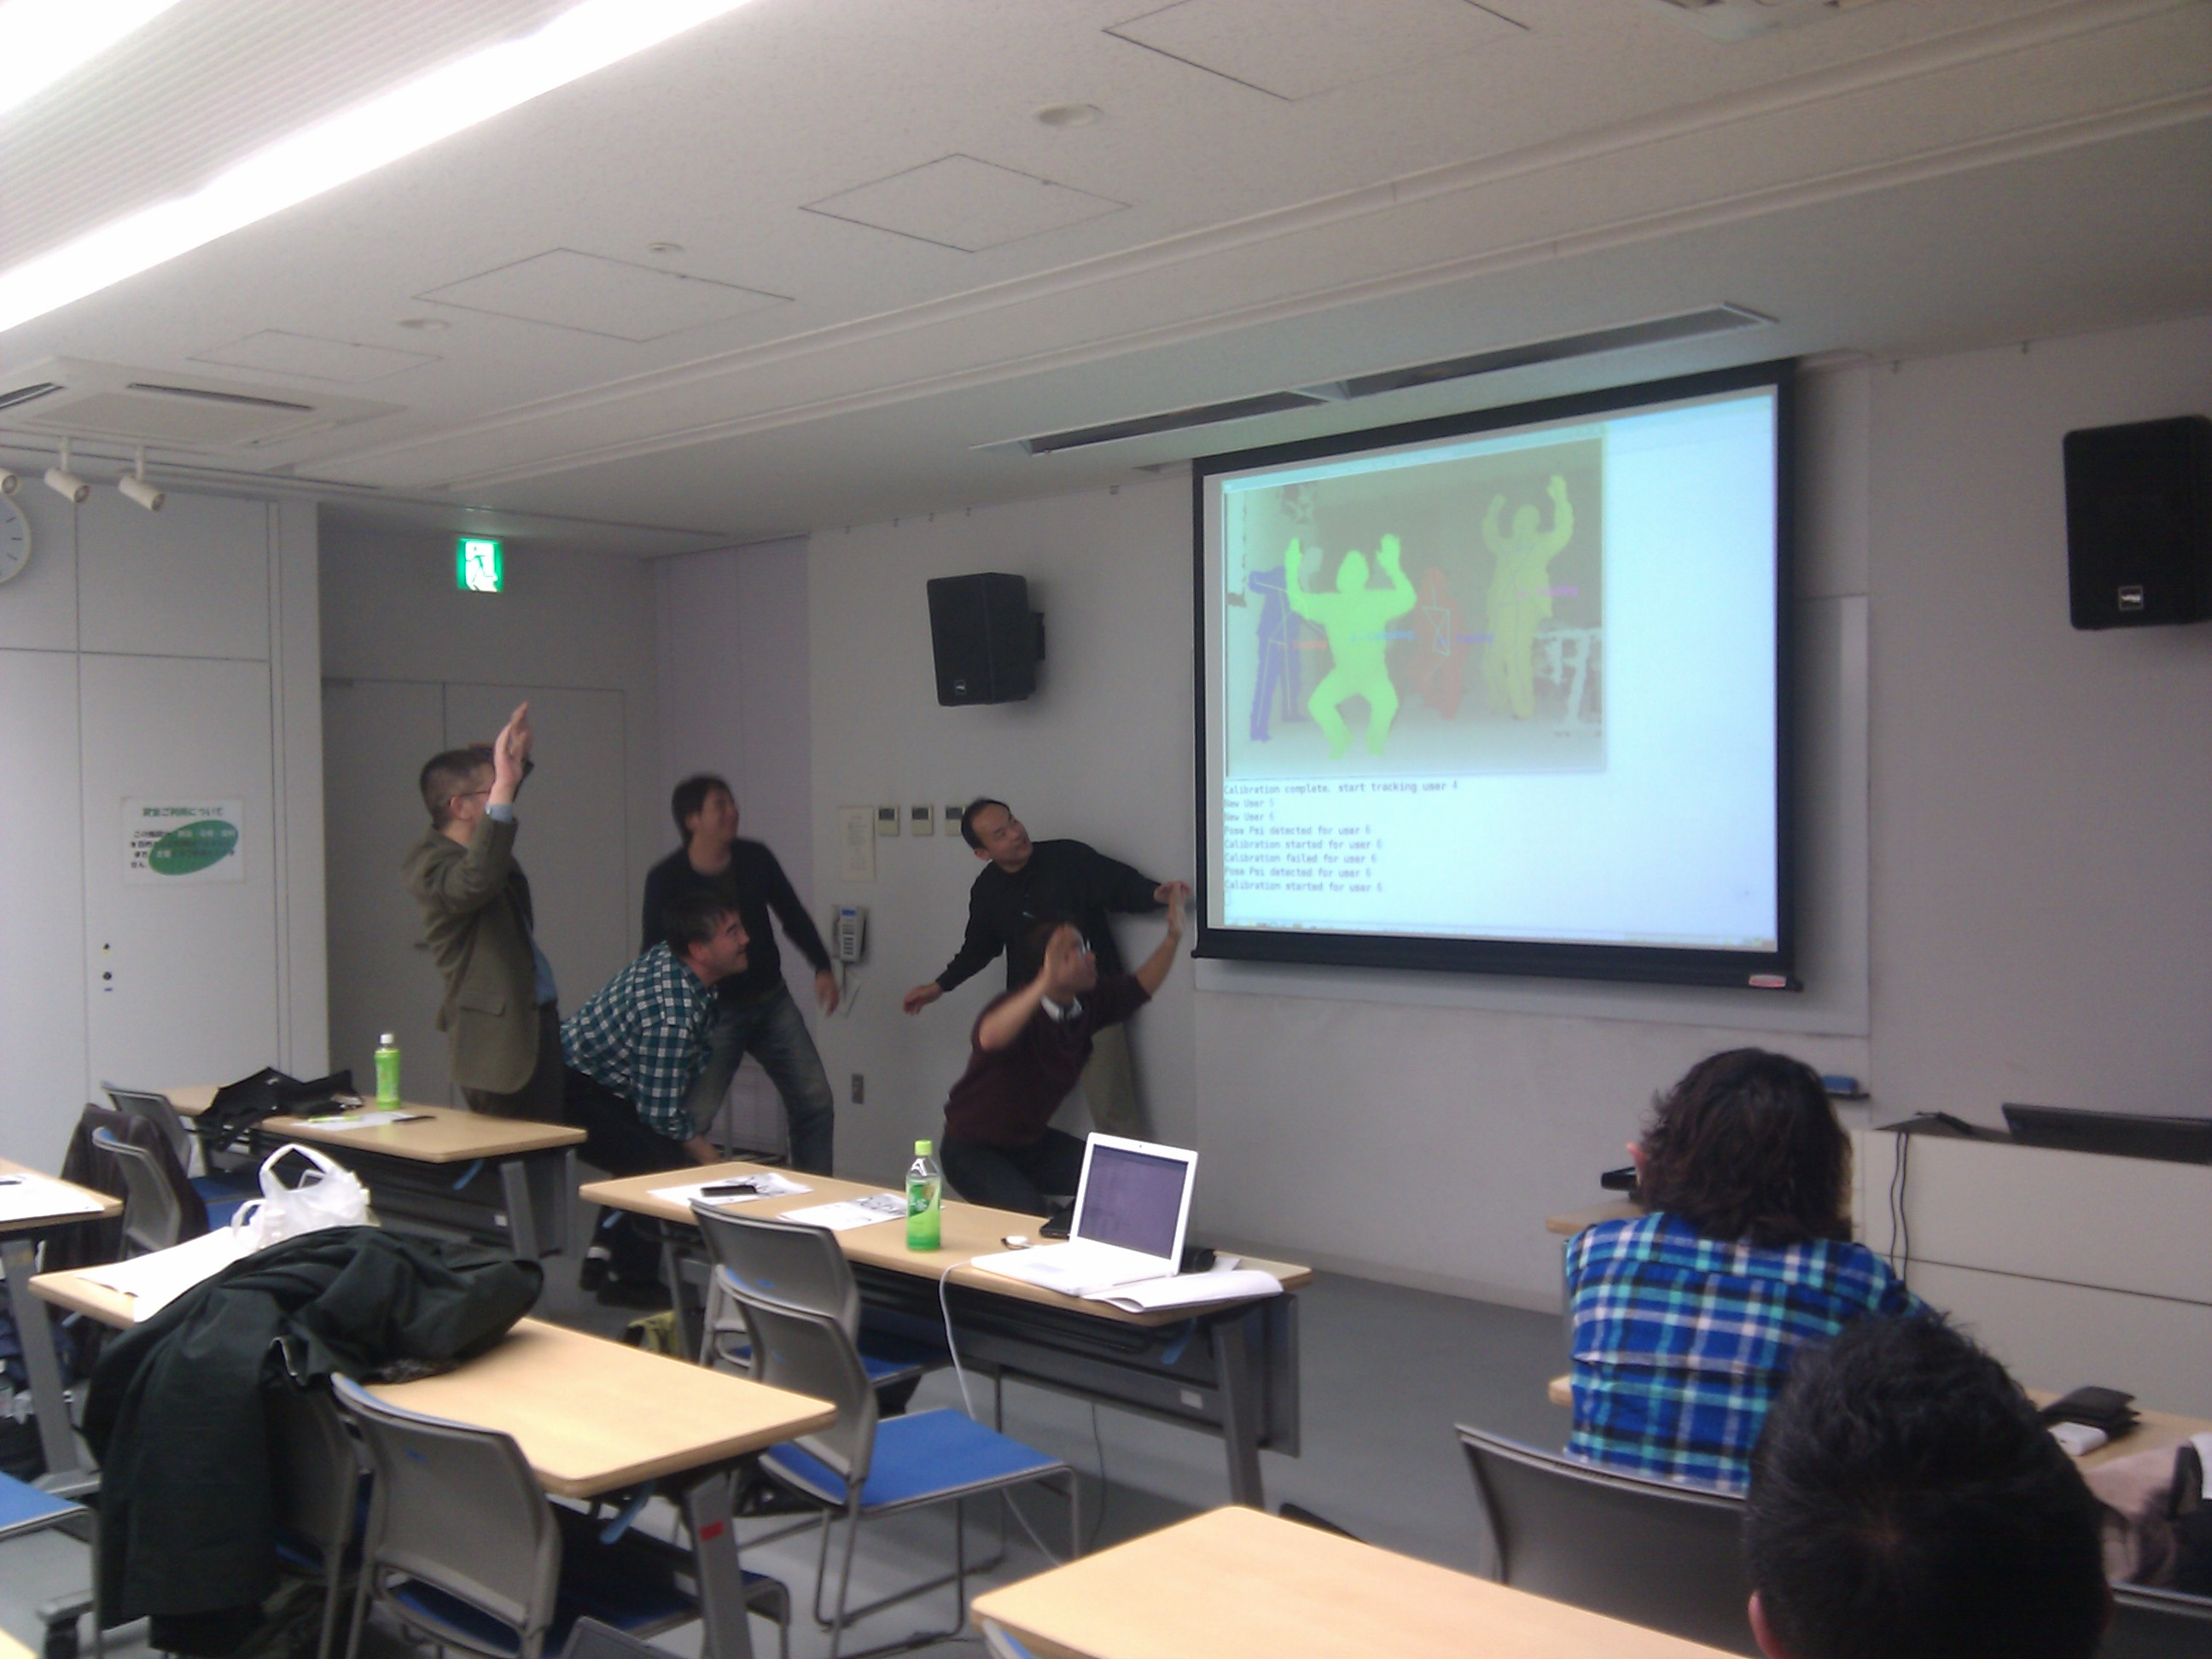
\includegraphics[width=.5\textwidth]{./image201101/kinect.jpg}
\end{frame}



\section{事前課題発表}


\takahashi[50]{事前課題}


\begin{frame}[fragile]
\frametitle{今回の事前課題}

\begin{block}{ nogajun による reportbug 解説の予習もかねて}
一つバグをみつけてきて下さい. ご意見要望でもかまいません.
\end{block}


\end{frame}


\takahashi[50]{事前課題\\発表}


\begin{frame}[fragile]
\frametitle{ 甲斐正三 }
  \begin{description}
  \item [未解決事項(私にとって)] \\
    texworksにおいて日本語が使用できない。
  \item [環境]
    Debian squeeze,texworks ver0.2.3
  \item [補足]
    バグなのか、設定が適正でないからなのかわかっていません。
  \item [今後の予定]
    他のdistroでも同様なのか確認してみます。
  \item [Texの用途]
    タイミングチャート(図)を含む文章を整形したい。
  \end{description}
\end{frame}

\begin{frame}[fragile]
\frametitle{ かわだてつたろう }

当日までに何かみつけます。。。

\end{frame}

\begin{frame}[fragile]
\frametitle{ 山田 洋平 }

去年、はじめてバグを報告し、パッケージを修正してもらえました。
今回は要望を挙げてみたいと思います。日本語環境を改善したいので、当日までに状況を調べて来ます。

\end{frame}

\begin{frame}[fragile]
\frametitle{ 八津尾 }

要望: Anthyの学習量上限を増やして欲しいなぁ

\end{frame}

\begin{frame}[fragile]
\frametitle{ dictoss(杉本 典充) }

kfreebsd-amd64環境で、iceweaselで使っているときにハイパーリンク部のテキストをクリックするとフリーズする場合がある。このとき、タブの読み込み中のくるくる回るアニメーションもフリーズする。
\end{frame}



\begin{frame}[fragile]
\frametitle{ 佐々木洋平 }
\begin{itemize}
\item
  yaskkserv: daemon が動作していない時に /etc/init.d/yaskkserv restart すると error
\end{itemize}
    \begin{commandline}
% sudo /etc/init.d/yaskkserv stop
% sudo /etc/init.d/yaskkserv restart
Restarting yaskkserv: yaskkservkill: 297: Usage: kill [-s sigspec | -signum | -sigspec] [pid | job]... or
kill -l [exitstatus]
    \end{commandline}
    \begin{itemize}
    \item howm: howm-vars.el で old-style backqoutes
    \item elscreen: emasc22 以降, elscreen 使うと起動時にファイルが開けません.
    \item ptex-base,ptex-bin (wishlist): UTF-8 が通りません.
    \end{itemize}
\end{frame}

\begin{frame}[fragile]
\frametitle{ dpqpqb }

lenny のシャットダウン中にハングする場合が有る.
仕方無しに電源ボタンの長押しで対処してます.
\begin{itemize}
\item Debian 5.0.8
\item Kernel 2.6.26-2-686
\item GNOME  2.22.3
\end{itemize}
\end{frame}

\begin{frame}[fragile]
\frametitle{ 山下康成 }

\url{http://www.debian.org/releases/squeeze/armel/apds03.html.ja}
D.3.4.1. デバイスファイルの作成 には,
\begin{commandline}
次のようにして, デフォルトの静的デバイスファイル群を作成します.

# cd /dev
# MAKEDEV generic
\end{commandline}
との記述がありますが, 記述の通りに実行すると,
\begin{commandline}
# MAKEDEV generic
.udevdb or .udev presence implies active udev.  Aborting MAKEDEV invocation.
#
\end{commandline}
となります
\end{frame}

\begin{frame}[fragile]
\frametitle{ 川江 }

バグについてですが, 以前にも話した事があるようにスクリプトやパッケージが自分の「意図」と異なる動きをしたときに, それが「バグ」なのか「設定ミス」なのか分からないときがあります. Xen で言えば時刻の設定や iptables で forward を有効に設定した場合に各 DomainU が外部に接続できなくなるなどです.
\end{frame}

\begin{frame}[fragile]
\frametitle{ 松澤二郎 }

reportbug がローカライズされていない. gettext のラッピングさえしてなさげ.
(むしろ意図的? 当然英語を使えよな, と暗にほのめかしている気もする)
\end{frame}

\begin{frame}[fragile]
\frametitle{ bpasao }

(無回答)

\end{frame}

\begin{frame}[fragile]
\frametitle{ lurdan }

{\url{http://bugs.debian.org/cgi-bin/bugreport.cgi?bug=607721}}

ITP のサンプルです.
\end{frame}

\begin{frame}[fragile]
\frametitle{ のがたじゅん }

gpsbabel-gui パッケージで desktop ファイルがないのでメニューに反映されない.

\end{frame}


\takahashi[50]{そんな\\こんなで}
\takahashi[120]{次}

\section{Debian GNU/kFreeBSD で便利に暮らすための Tips by 杉本典充}

\takahashi[25]{Debian GNU/kFreeBSD で\\便利に暮らすための Tips \\by\\杉本典充}

\takahashi[50]{そんな\\こんなで}
\takahashi[120]{次}

\section{バグ報告はバグのためだけじゃないよ  by のがたじゅん}

\takahashi[25]{バグ報告はバグのためだけじゃないよ \\ by \\ のがたじゅん}

\takahashi[50]{そんな\\こんなで}
\takahashi[120]{次}

\begin{frame}[fragile]
\frametitle{今後の予定}


\begin{block}{第 44 回関西 Debian 勉強会}
\begin{itemize}
  \item 日時: 2 月 26 日
  \item 会場: 未定
  \item 内容: 未定
  \begin{itemize}
    \item 多分リリースされてるよね
    \item OSC 神戸の事, そろそろ決めようよ
  \end{itemize}
\end{itemize}
\end{block}


\end{frame}



\takahashi[50]{  }


\end{document}
%%% Local Variables:
%%% mode: japanese-latex
%%% TeX-master: t
%%% End:
